\documentclass[master=cws,masteroption=se]{kulemt}
\setup{title={DevOps: Operational data for developers},
  author={Stef Van Gils},
  promotor={Prof.\ W. Joosen},
  assessor={Dimitri Van Landuyt},
  assistant={Dimitri Van Landuyt}}
% De volgende \setup mag verwijderd worden als geen fiche gewenst is.
\setup{filingcard,
  translatedtitle={DevOps: Operational data for developers},
  udc=621.3,
  shortabstract={}}
% Verwijder de "%" op de volgende lijn als je de kaft wil afdrukken
%\setup{coverpageonly}
% Verwijder de "%" op de volgende lijn als je enkel de eerste pagina's wil
% afdrukken en de rest bv. via Word aanmaken.
%\setup{frontpagesonly}

% Kies de fonts voor de gewone tekst, bv. Latin Modern
\setup{font=lm}

% Hier kun je dan nog andere pakketten laden of eigen definities voorzien

% Tenslotte wordt hyperref gebruikt voor pdf bestanden.
% Dit mag verwijderd worden voor de af te drukken versie.
\usepackage[pdfusetitle,colorlinks,plainpages=false]{hyperref}
\usepackage{url}
%%%%%%%
% Om wat tekst te genereren wordt hier het lipsum pakket gebruikt.
% Bij een echte masterproef heb je dit natuurlijk nooit nodig!
\IfFileExists{lipsum.sty}%
 {\usepackage{lipsum}\setlipsumdefault{11-13}}%
 {\newcommand{\lipsum}[1][11-13]{\par Hier komt wat tekst: lipsum ##1.\par}}
%%%%%%%

%%%%%%%
% Gebruikt om \texttt{} line breaks uit te voeren indien nodig
\newcommand*\justify{%
  \fontdimen2\font=0.4em% interword space
  \fontdimen3\font=0.2em% interword stretch
  \fontdimen4\font=0.1em% interword shrink
  \fontdimen7\font=0.1em% extra space
  \hyphenchar\font=`\-% allowing hyphenation
}
%%%%%%%

%\includeonly{hfdst-n}
\begin{document}

\begin{preface}
  Dit is mijn dankwoord om iedereen te danken die mij bezig gehouden heeft.
  Hierbij dank ik mijn promotor, mijn begeleider en de voltallige jury.
  Ook mijn familie heeft mij erg gesteund natuurlijk.
\end{preface}

\tableofcontents*

\begin{abstract}
  In dit \texttt{abstract} environment wordt een al dan niet uitgebreide
  samenvatting van het werk gegeven. De bedoeling is wel dat dit tot
  1~bladzijde beperkt blijft.

  \lipsum[1]
\end{abstract}

% Een lijst van figuren en tabellen is optioneel
%\listoffigures
%\listoftables
% Bij een beperkt aantal figuren en tabellen gebruik je liever het volgende:
\listoffiguresandtables
% De lijst van symbolen is eveneens optioneel.
% Deze lijst moet wel manueel aangemaakt worden, bv. als volgt:

% Nu begint de eigenlijke tekst
\mainmatter

%\chapter{Inleiding}
\label{inleiding}
In dit hoofdstuk wordt het werk ingeleid. Het doel wordt gedefinieerd en er
wordt uitgelegd wat de te volgen weg is (beter bekend als de rode draad).

Als je niet goed weet wat een masterproef is, kan je altijd
Wikipedia\cite{wiki} eens nakijken.

\section{Lorem ipsum 4--5}
\lipsum[4-5]

\section{Lorem ipsum 6--7}
\lipsum[6-7]

%%% Local Variables: 
%%% mode: latex
%%% TeX-master: "masterproef"
%%% End: 

%\include{hfdst-1}
\chapter{Context}

\section{Relevantie monitoren mobiele applicaties}
Op het moment van schrijven is het 2016; het jaar waarin ongeveer \'e\'en op de vijf mensen een smartphone gebruikt in het dagelijkse leven. Een smartphone bevat meerdere mobiele applicaties, ontwikkeld door developers wereldwijd. In de App Store van Apple staan ongeveer 1.5 miljoen verschillende applicaties. Een karakteristiek van de mobiele app wereld is dat er voor een bepaalde app vaak een of meerdere alternatieven bestaan. Dit wil zeggen dat de eigenaars van de app zich moeten proberen onderscheiden van de andere apps. Dat kan op meerdere manieren: door een praktisch design, door een snellere app te hebben, etc. Door tijd en/of geld te investeren in het verbeteren van de applicatie kan de applicatie de meest gebruikte applicatie worden en blijven in zijn categorie. \\
%cite http://www.statista.com/statistics/330695/number-of-smartphone-users-worldwide/

Met het design wordt de structuur van de gebruikersinterface van de applicatie bedoeld. Dit design bepaalt waar welke UI elementen komen te staan. Er wordt hier niet bedoeld op de esthetiek van de gebruikersinterface.
Het design wordt meestal op voorhand vastgelegd alvorens de applicatie ontwikkeld wordt, zodat de developer dit kan gebruiken bij het implementeren. Er kan niet objectief gezegd worden wat een goed of een slecht design is door een ontwikkelaar omdat dit een persoonlijke mening is. Het design kan enkel \'echt beoordeeld worden door de gebruikers van de applicatie. Dit komt omdat er een verschil kan zijn in hoe de eigenaars van de applicatie denken dat de applicatie gebruikt wordt en in hoe de gebruikers de applicatie gebruiken. Als er een verschil in deze denkwijze zit, dan zou het design best aangepast worden naar de smaak van de gebruikers. Dit bevordert enerzijds de kwaliteit van de applicatie en anderzijds cre\"eert het een band tussen gebruiker en developer. Indien er geen input komt van de gebruikers kan het nog steeds zijn dat de applicatie niet gebruikt wordt hoe de eigenaar het denkt. Er moet dan ontdekt worden welke elementen gebruikt worden en welke niet. Het monitoren van deze elementen kan ervoor zorgen dat er een goed beeld gevormd wordt voor de eigenaar die met deze informatie zijn inzicht in de applicatie kan veranderen. Dit zorgt ervoor dat de eigenaar betere beslissingen kan maken omtrent de toekomst en de verdere ontwikkeling van de applicatie. Zelfs al zijn er reviews van de gebruikers, dan nog is het voor de eigenaar meestal onmogelijk om te ontdekken welke elementen in de applicatie gebruikt worden en welke niet. Het is dus belangrijk om de applicatie te monitoren, ookal is er veel input van de gebruikers. \\


De prestaties van een applicatie zijn belangrijk voor een eigenaar omdat deze een impact hebben op de gebruiksvriendelijkheid van de applicatie. De meeste problemen die te maken hebben met prestaties zijn op te lossen door voldoende testen te schrijven en hiermee bugs en trage code sequenties uit de code te halen, maar sommige prestatie problemen doen zich enkel voor bij een significant gebruikersaantal. Drie uit de top tien van meest vermelde klachten van mobiele applicaties hebben te maken met de prestaties van een applicatie, namelijk: \textit{Resource-Heavy, Slow or lagging} en \textit{Frequent Crashing}. Deze klachten worden vaak in reviews van gebruikers geuit. De eigenaars kunnen hieruit opmaken dat er een probleem is, maar developers weten niet zeker waar het fout loopt uit die reviews. Om uit te vinden waar de prestatie problemen zitten is het voor de developers handig om de applicatie te monitoren waar de bottlenecks kunnen ontstaan. Hierdoor kunnen ze de exacte oorzaak van het probleem vinden. Op deze manier kan een potenti\"eel probleem al ontdekt worden voor deze in de reviews van de gebruikers opduikt. Dit zorgt ervoor dat de tevredenheid niet naar beneden gaat, omdat het probleem op voorhand al ontdekt wordt. \\
%cite http://appealingstudio.com/why-your-app-sucks-the-20-most-common-complaints-about-mobile-apps-2/


De reviews die door de gebruikers worden gelezen moeten met een korrel zout genomen worden; mensen hebben de intentie om te overdrijven. De eigenaars kunnen hiervoor gebruik maken van een methode, ontwikkeld door de Carnegie Mellon Universiteit, die een analyse uitvoert van deze reviews en de inconsistente reviews eruit filtert. Zo kan er een goed standpunt gevormd worden rond de kwaliteit van de applicatie. Maar zelfs met die methode zijn reviews nog steeds subjectief als het gaat over prestaties. De enige manier om objectief te redeneren hierover is door middel van metingen uit te voeren. Deze metingen kunnen ge\"implementeerd worden door de developer zelf of door een monitoring library. Het gebruik van een monitoring library brengt vele voordelen met zich mee ten opzichte van het zelf implementeren van een systeem. Een monitoring library is ontwikkeld met als doel het zo goed mogelijk monitoren van een applicatie en heeft dus alle diensten hiervoor in huis. De tijd en moeite die een developer in het monitoren van een applicatie steekt is significant lager dan dat de developer zelf nog een systeem moet implementeren. Dit komt omdat de monitoring library klaar is om gebruikt te worden en alle communicatie in deze library verwerkt is, terwijl een developer zelf nog deze communicatie zou moeten schrijven en een back end. Een monitoring library zorgt voor het verwerken en het weergeven van deze data in grafieken zodat er een goed beeld hiervan gevormd kan worden. Een nadeel van een externe monitoring library te gebruiken is dat de data opgeslagen staat op de servers van de externe partij en dat deze in vele gevallen niet opgevraagd kan worden bij die partij. Een ander nadeel is dat de developer de data anders of dieper wil analyseren dan dat gebeurt in de monitoring library. De eigenaars moeten dus een keuze maken tussen het ontwikkelen van een eigen, nieuw, monitoring systeem waar veel tijd en moeite in kruipt en waarvoor voldoende infrastructuur voor moet voorzien worden (back end servers) en het in gebruik nemen van een bestaande monitoring library die misschien net niet genoeg functionaliteit voorziet of de data niet beschikbaar stelt aan de eigenaars van de applicatie.\\
%cite de paper van de universiteit


Het monitoren van mobiele applicaties is anders dan het monitoren van websites, internet applicaties en pc applicaties omwille van een aantal factoren. Een mobiele applicatie draait op een besturingssysteem dat speciaal ontworpen is voor de mobiele telefoons. Android en iOS zijn de twee besturingssystemen die het waard zijn om te vermelden. Een mobiele applicatie wordt dus meestal voor beiden ontwikkeld om een zo groot mogelijk aantal gebruikers te bereiken. Ontwikkelen voor de andere besturingssystemen is meestal niet rendabel voor de moeite en het geld dat erin moet gestoken worden. De monitoring library draait dus maar op twee verschillende systemen, terwijl er tientallen web browsers bestaan waar websites en internet applicaties in draaien. \\
%cite android en ios market share
Indien de applicaties native worden ontwikkeld, dan moet de applicatie een keer voor Android en een keer voor iOS ontwikkeld worden. Dit zorgt ervoor dat er verschillende bugs en/of bottlenecks in de verschillende applicaties kunnen zitten. Het zou verkeerd zijn om gecollecteerde data van de twee applicaties samen te verwerken. \\
Een desktop computer of laptop heeft in de meeste gevallen ofwel een WiFi verbinding of een ethernet verbinding met het internet. De internetverbinding van een smartphone varieert tussen WiFi en een mobiel netwerk (4G, 3G, Edge, ...). Deze connecties hebben een verschillende snelheid en moeten dus anders ge\"interpreteerd worden. \\

Bij het monitoren van mobiele applicaties is het noodzakelijk dat een monitoring library zo weinig mogelijk resources (CPU, batterij, netwerk) gebruikt. Zoals eerder al vermeld is dit \'e\'en van de meest voorkomende klachten bij gebruikers van een mobiele applicatie. Bij pc applicaties wordt hier bijna nooit rekening mee gehouden, omdat de prestaties van de resources hier significant hoger zijn dan bij smartphones. Bij internet applicaties is dit niet van toepassing, omdat dit heel erg af hangt van de implementatie van de browser. \\


Het monitoren van mobiele applicaties is op veel vlakken een handige feature. Enerzijds om als ondersteuning te dienen voor de eigenaars om de gebruikers van de applicatie tevreden te stellen en de applicatie te kunnen verbeteren/veranderen in functie van de gebruiker en hoe de applicatie gebruikt wordt. Anderzijds dient het monitoren van de applicatie als een hulpmiddel voor de developers om te kunnen ontdekken of er bugs in de applicatie zitten en ook de plaats van voorkomen te identificeren zodat deze opgelost kunnen geraken in een volgende versie. Er moet een keuze gemaakt worden tussen het gebruik van een bestaand monitoringsysteem of het zelf ontwikkelen van zo'n systeem met alle voordelen en nadelen in rekening gebracht. \\


\section{Development Scenarios}
In deze sectie worden een aantal scenarios geschetst waar een developer of eigenaar er baat bij heeft om een monitoring library te gebruiken. 

\subsection{General Purpose App}
Een general purpose app is een mobiele applicatie die geen game is (bv. Facebook, Shazam, maar ook een gewone camera app). De functionaliteiten van deze applicaties zijn heel uiteenlopend. Een eigenaar en een developer hebben verschillende informatie nodig om beslissingen omtrent de applicatie te nemen. Deze worden daarom in de volgende paragrafen afgezonderd.
%cite facebook, shazam

\paragraph{Eigenaar}
Een eigenaar wil dat de applicatie zoveel mogelijk gebruikt wordt en zoveel mogelijk geld opbrengt (door bv. advertenties). Om gebruikers te lokken en deze ook te houden moet de eigenaar de applicatie af en toe updaten om gegeerde features toe te voegen of te verbeteren en niet gebruikte features te verwijderen. Zonder een of ander monitorsysteem is het voor de eigenaar bijna onmogelijk om te weten welke features vaak gebruikt worden en welke niet. 

Indien de eigenaar weet welke onderdelen vaak gebruikt worden kan hij hierop inspelen door goed geplaatste advertenties in de applicatie in te bouwen en hiermee geld te verdienen. Het beste zou dan zijn om het onderdeel uit de applicatie te halen. Indien een onderdeel zelden gebruikt wordt is het niet voordelig om dit onderdeel te blijven ondersteunen of verbeteren. Het zou beter zijn om dit uit de applicatie te verwijderen.

De eigenaar kan het design van de applicatie aanpassen om een weinig gebruikt onderdeel meer in de spotlight te zetten zodat gebruikers dit vaker zouden gebruiken. \\


\paragraph{Developer}
De eigenaar wil vooral weten hoe de applicatie gebruikt wordt. De developer wil vooral weten of de applicatie naar behoren werkt en er geen bugs of bottlenecks in zitten. De meeste bugs zouden er in de testfase uitgehaald moeten worden, maar er zijn bugs en bottlenecks die enkel op grote schaal zichtbaar zijn. Meestal heeft dit te maken met het ontvangen of verzenden van content over het netwerk, maar kan ook te maken hebben met het lokaal verwerken van data. Zonder een monitorsysteem is het voor de developers in vele gevallen een hele uitdaging om de bottleneck of de bug te vinden. Met een monitorsysteem kunnen de developers op bepaalde kritieke punten metingen uitvoeren. Indien er dan een bottleneck aanwezig is in de applicatie, dan weten de developers op welk punt het fout loopt. Hierdoor wordt er veel tijd bespaard in het zoeken naar deze bottleneck. \\



\subsection{Game}
De game die besproken wordt is het populaire spel \textbf{Angry Birds}. In dit spel krijgt een speler drie beurten om alle vijanden te verslaan door een constructie omver te werpen en de vijanden schade te berokkenen. Indien alle vijanden verslagen zijn eindigt het level en krijgt de speler een score en een beoordeling van maximaal drie sterren. Dit scenario wordt alsook opgedeeld in een beschrijving van de voordelen voor de eigenaar en voor een developer.
%cite angry birds

\paragraph{Eigenaar}
De eigenaar wil ervoor zorgen dat de applicatie zoveel mogelijk gebruikt wordt en dat de levels niet te moeilijk, maar ook niet te gemakkelijk zijn. Om te kijken dat de levels niet te moeilijk zijn kan de eigenaar de developers vragen om per level bij te houden hoe vaak er op de reset toets gedrukt is, hoeveel sterren de spelers gemiddeld verzamelen en hoeveel beurten er gemiddeld gebruikt worden. Hieruit kan de eigenaar dan opmaken of de levels de gewenste moeilijkheidsgraad hebben en in de toekomst deze getallen mee in rekening te nemen in het ontwikkelen van nieuwe levels.

De populariteit van een spel hangt vaak af hoe vaak het gespeeld wordt en hoe lang een spelsessie duurt. Dit kan gemeten worden met een monitoring library door elke keer dat de applicatie gestart wordt dit door te sturen naar de server en een timer te starten die stopt wanneer de gebruiker de app sluit. De eigenaar kan zo ingrijpen als de app minder (lang) gebruikt wordt dan voorheen door zelf te adverteren of andere initiatieven. \\

\paragraph{Developer}
De developer wil vooral op de hoogte zijn van de prestaties van de applicaties en eventuele bugs vinden. Bij Angry Birds heeft dit impact op twee verschillende situaties, namelijk de periode dat de gebruiker zich in het menu bevindt en de periode dat de gebruiker het spel speelt. Het verschil hierin is wat er gemonitord wordt. In het spel zelf is het belangrijk dat de framerate niet te laag wordt. De developer zal dit dan ook monitoren in het spel zelf. In het menu is dit minder belangrijk. Hier is het eerder belangrijk dat er geen significante vertragingen oplopen in het navigeren door de menu's en de verschillende collecties van levels.\\


Deze development scenarios tonen aan dat het gebruik van een monitoring library in mobiele applicaties niet alleen de developer, maar ook de eigenaar kan helpen in het maken van beslissingen omtrent de applicatie. Op deze manier kan er data verzameld worden wanneer de applicatie al in de handen is van de gebruikers. Dit staat tegenover een testomgeving die meestal enkel op kleine schaal uitgevoerd wordt.







\chapter{Doelstelling} \label{doelstelling}
Het onderzoek van deze thesis baseert zich op twee invalshoeken, enerzijds hoe de developers en eigenaars van een mobiele applicatie geholpen kunnen worden bij het ontwikkelen en verbeteren van die applicatie en anderzijds wat de trade-off is tussen enerzijds hoeveel de applicatie gemonitord wordt en anderzijds de impact op de performance van de applicatie, de developer effort, etc. \\

De eerste invalshoek gaat over hoe we developers kunnen helpen bij het ontwikkelen van een mobiele applicatie door de developers problemen te laten identificeren (zoals trage code sequenties) en de eigenaars te laten ontdekken welke componenten van de applicatie het meest gebruikt worden en welke het minste. Met deze informatie weten de developers waar ze verbeteringen kunnen aanbrengen en weten eigenaren in welke functies ze wel of niet moeten investeren. Langs de andere kant is het belangrijk om te weten wat de impact is van het verkrijgen van de informatie op de prestaties van de applicatie en hoeveel moeite en tijd er nodig is van de developer om deze informatie te kunnen vergaren.\\


Om dit onderzoek te doen slagen wordt er een library gebouwd die developers in hun applicaties kunnen inbouwen om hun applicatie te monitoren. In de volgende sectie wordt uitgelegd wat het doel is van deze library. In het verdere verloop van deze thesis wordt uitgelegd hoe de architectuur achter de gebouwde library in elkaar zit en waarom de keuzes zijn gemaakt voor die structuur. Nadat deze architectuur beschreven is wordt er een uitleg gegeven over de specifieke implementatie van de library. Ten slotte wordt de library ge\"evalueerd om te kijken of de kwaliteit van de library voldoende is om gebruikt te worden in de applicaties. 

\section{Library}
Het doel van de library is om developers deze library te laten inbouwen in hun applicatie en met behulp van de methodes aangeboden door deze library de applicatie te kunnen monitoren. Deze methodes moeten voldoende zijn om alle aspecten van de applicatie te kunnen monitoren. \\

Om een kwaliteitsvolle library te bouwen zijn er een aantal aspecten die belangrijk zijn om in het achterhoofd te houden:
\begin{itemize}
\item performance impact
\item schaalbaarheid
\item bruikbaarheid
\item beschikbaarheid
\end{itemize}

Deze aspecten worden besproken in het komende deel van dit hoofdstuk. 

\subsection{Performance impact}
Het is van cruciaal belang dat een applicatie niet traag is en responsief is naar de gebruiker toe. De verwerkingskracht (CPU) van een mobiel apparaat is relatief beperkt. Deze twee eigenschappen gecombineerd zorgt ervoor dat de library een zo beperkt mogelijke impact mag hebben op deze verwerkingskracht. Indien deze library relatief veel CPU tijd inneemt, dan blijft er minder CPU tijd over voor de applicatie, wat ervoor zorgt dat de applicatie trager wordt indien deze CPU-intensief is. Het is dus van cruciaal belang dat de library geoptimaliseerd wordt om zo weinig mogelijk CPU tijd te verbruiken. Een bijkomend voordeel dat verschijnt indien de library zo minimaal mogelijk CPU tijd verbruikt is dat de impact van de applicatie op het batterijverbruik verminderd wordt.  \\

Naast het CPU verbruik is het ook van belang dat het netwerkgebruik zo effici\"ent mogelijk gebruikt wordt. In een mobiel apparaat wordt de netwerkinterface in slaapstand gehouden tot deze gebruikt moet worden en op dat moment wordt deze interface geactiveerd. Dit wordt gedaan omdat de netwerkinterface relatief veel energie verbruikt indien deze aanstaat. Indien de netwerkinterface zo effici\"ent mogelijk gebruikt wordt kan deze vaker in slaapstand gezet worden en is de impact van de library op het batterijgebruik minder dan indien deze ineffici\"ent gebruikt wordt. Deze effici\"entie zorgt er ook voor dat de applicatie de netwerkinterface zo vaak mogelijk kan gebruiken en hier zo weinig mogelijk vertraging opgelopen wordt als de applicatie het netwerk wil gebruiken. \\

Niet enkel de effici\"entie van het gebruik van de netwerkinterface is van belang, maar ook de snelheid waarmee de back end reageert op de request en deze een resultaat kan terug geven. Indien het relatief lang duurt eer de back end het resultaat terug geeft, is de optimalisatie van het gebruik van de netwerkinterface voor niets geweest. De snelheid van de back end is dus ook een belangrijk aspect. \\

De impact op de performance van de applicatie is het belangrijkste aspect in het bouwen van een monitoring library voor mobiele applicaties. Indien deze impact relatief groot is, dan is het voor developers onmogelijk om deze library in de applicatie in te bouwen en nog steeds een degelijke responsiviteit en snelheid van deze applicatie te behalen. 

\subsection{Schaalbaarheid}
Zoals hierboven vermeld is de snelheid van de back end een belangrijk aspect inzake performance van de netwerkinterface. \'E\'en aspect van deze snelheid is de implementatie van deze back end. De implementatie moet geoptimaliseerd worden zodat deze zo snel mogelijk een resultaat kan teruggeven aan de library. Het andere aspect in de snelheid van de back end is de load die de servers aankunnen om al de requests te verwerken. De mate van schaalbaarheid is hier een belangrijke factor in. \\

Een applicatie wordt simultaan gebruikt door gemiddeld \textit{N} gebruikers waarin de library aanwezig is. Deze applicatie verstuurt per keer gemiddeld \textit{X} metingen. De library wordt gebruikt door \textit{M} verschillende applicaties. De applicaties zijn geconfigureerd met een gemiddeld synchronisatie-interval \textit{T}. Dit geeft dat het gemiddeld aantal requests per tijdseenheid neerkomt op: $RpT=\frac{M*N*X}{T}$. Hoe hoger dit getal, hoe hoger het aantal requests de servers moeten beantwoorden en hoe meer load er per server komt. Elke server \textit{S} heeft een limiet kwa aantal requests die simultaan kunnen beantwoord worden \textit{R}. De volgende vergelijking geeft de relatie aan tussen het gemiddeld aantal requests en het aantal requests dat beantwoord kan worden: $S*R > RpT$. Dit wil zeggen dat er (altijd) meer requests moeten kunnen beantwoord worden dan dat er gemiddeld per tijdseenheid aan komen.\\



\subsection{Bruikbaarheid}
Het primaire doel van een library is om de taken uit te voeren die worden gegeven aan de library. Naast dit primaire doel is het ook de bedoeling dat developers de library kunnen gebruiken zonder veel effort. De bruikbaarheid van de library moet zo hoog mogelijk zijn zodat developers zonder veel tijd en moeite deze kunnen integreren in een applicatie. De volgende punten zijn hierin belangrijk: 

\begin{itemize}
\item Concreet willen we maximaal vermijden dat de library de developer hindert bij het ontwikkelen van de applicatie.

\item Concreet hebben we als doelstelling het vereiste aantal lijnen code en configuratie zo klein mogelijk te houden.

\item Concreet willen we dat de developer een zo minimaal mogelijke tijd moet spenderen bij het implementeren van de library.
\end{itemize}




\subsection{Beschikbaarheid}
Met beschikbaarheid wordt bedoeld dat alle gecollecteerde data opgeslagen wordt op de servers. De data die gecollecteerd wordt is waardevol. Het is de bedoeling dat er zo'n goed mogelijk beeld geschetst wordt voor de developer. Indien een deel van de data niet opgeslagen wordt in de database kan het zijn dat mogelijke uitzonderlijke data niet opgeslagen wordt, terwijl deze uitzonderlijke data juist de belangrijkste is. Er moet dus voor gezorgd worden dat 100\% van de gecollecteerde data gesynchroniseerd wordt naar de server om een zo goed mogelijk beeld te vormen voor de developers en de eigenaars van de applicatie.\\


Deze aspecten moeten in rekening genomen worden bij het ontwerpen en ontwikkelen van een mobiele monitoring library. De belangrijkste aspecten zijn de performance aspecten, omdat in mobiele applicaties de verwerkingskracht en batterij de bottlenecks zijn. 


\section{Data Visualisatie}
Data visualisatie is een belangrijk aspect in de library, omdat de developer uit deze visualisaties conclusies moet kunnen trekken over de prestaties en het gebruik van de applicatie. De verzamelde data van de gebruikers is samengenomen in \'e\'en centraal punt. Het doel is om deze data samen te voegen en hieruit de nodige informatie te halen en weer te geven aan de developer. Het is dus de zaak om uit te zoeken voor elk soort meting welke informatie belangrijk is. Deze informatie moet worden gevisualiseerd om de developer een compacter overzicht te geven van de resultaten van de metingen. Door de data te groeperen op eigenschappen kan de developer dieper ingaan op de details van de metingen. Indien er niet aan data visualisatie gedaan zou worden, zou de developer zelf de verschillende parameters moeten berekenen uit de ruwe data. \\

Het uiteindelijke doel is dus om per type meting de parameters te gaan identificeren die nuttig kunnen zijn voor de developer om een conclusie uit dat type meting te kunnen trekken. Daarnaast is het de bedoeling om een software pakket te maken die deze parameters gaat weergeven in een overzicht voor de developer.

%%% Local Variables: 
%%% mode: latex
%%% TeX-master: "masterproef"
%%% End: 

\include{architectuur} 
\include{implementatie}
\include{evaluatie}
% ... en zo verder tot
%\chapter{Het laatste hoofdstuk}
\label{hoofdstuk:n}
Een hoofdstuk behandelt een samenhangend geheel dat min of meer op zichzelf
staat. Het is dan ook logisch dat het begint met een inleiding, namelijk
het gedeelte van de tekst dat je nu aan het lezen bent.

\section{Eerste onderwerp in dit hoofdstuk}
De inleidende informatie van dit onderwerp.

\subsection{Een item}
De bijbehorende tekst. Denk eraan om de paragrafen lang genoeg te maken en
de zinnen niet te lang.

Een paragraaf omvat een gedachtengang en bevat dus steeds een paar zinnen.
Een paragraaf die maar \'e\'en lijn lang is, is dus uit den boze.

\section{Tweede onderwerp in dit hoofdstuk}
Er zijn in een hoofdstuk verschillende onderwerpen. We zullen nu
veronderstellen dat dit het laatste onderwerp is.

\section{Besluit van dit hoofdstuk}
Als je in dit hoofdstuk tot belangrijke resultaten of besluiten gekomen
bent, dan is het ook logisch om het hoofdstuk af te ronden met een
overzicht ervan. Voor hoofdstukken zoals de inleiding en het
literatuuroverzicht is dit niet strikt nodig.

%%% Local Variables: 
%%% mode: latex
%%% TeX-master: "masterproef"
%%% End: 

%\chapter{Besluit}
\label{besluit}


In deze thesis is er op zoek gegaan naar een oplossing om het ontwikkelen van mobiele applicaties en de concepten van DevOps te combineren. Er is gekozen om te kijken naar het monitoring aspect van DevOps. Er zijn enkele oplossingen voorgesteld om mobiele applicaties te monitoren, namelijk: built-in OS support, een dedicated test environment en een monitoring library. Uit deze voorstellen is \'e\'en voorstel gekozen, namelijk een library om in een mobiele applicatie in te bouwen die de applicatie monitort. In het doelstellingen hoofdstuk is beschreven welke specificaties de library minimaal moet hebben om een succesvolle library te kunnen zijn. De vormgeving en architectuur van de monitoring library wordt voorgesteld in het architectuur hoofdstuk samen met enkele uitbreidingen op de library. Deze architectuur is ge\"implementeerd in een library die ontwikkeld is voor iOS, het besturingssysteem voor mobiele toestellen van Apple. Deze implementatie is ten slotte ge\"evalueerd om te kijken of deze implementatie kan werken in de realiteit. \\


In het hoofdstuk doelstellingen \ref{doelstelling} zijn een aantal doelstellingen opgesomd voor de ontwikkelde library. Deze werden opgedeeld in volgende categorie\"en: 
\begin{itemize}
\item performance impact
\item schaalbaarheid
\item bruikbaarheid
\item beschikbaarheid
\end{itemize}

\paragraph{De performance impact} werd gezien als het belangrijkste aspect in het ontwikkelen van een monitoring library. Deze impact is onderzocht en getest in het evaluatie hoofstuk \ref{evaluatie}. Uit deze evaluatie kan afgeleid worden dat de impact van de library op een mobiele applicatie klein genoeg is om de applicatie niet significant te vertragen. \\


\paragraph{De schaalbaarheid} van de Tracklytics library is besproken in het evaluatie hoofdstuk \ref{evaluatie}. De back end is het deel van de library dat schaalbaar moet zijn om de requests die van de mobiele library komen te verwerken. De bottleneck in de back end is de relationele database. Deze moet zo goed mogelijk uitgeschaald worden om aan de requests te kunnen voldoen. Een alternatief is om de relationele database te veranderen naar een NoSQL of andere schaalbare database. Het is ook mogelijk voor de developer om de back end op de eigen servers te draaien om zo alle data in eigen bezit te hebben en niet afhankelijk te zijn van de Tracklytics infrastructuur.\\


\paragraph{De bruikbaarheid} van de library wordt gedefini\"eerd als hoeveel moeite een developer nodig heeft om de library in te bouwen in de mobiele applicatie. In het evaluatie hoofdstuk \ref{evaluatie} is nagegaan hoeveel moeite een developer nodig heeft om de library in de applicatie in te bouwen. In deze evaluatie zijn de volgende zaken opgenomen: de totale tijd om de library in te bouwen, het aantal lijnen code en wat er gemonitord wordt door de library. Uit de gegevens die hieruit zijn gekomen kan geconcludeerd worden dat de developer effort minimaal is.

\paragraph{Om de beschikbaarheid} van de data maximaal te houden moet elke meting naar de back end verstuurd worden. De Tracklytics library laat de keuze of de data tijdelijk op de harde schijf van het toestel opgeslagen moet worden over aan de developer zelf. De developer moet deze keuze aangeven in het dashboard. \\

De voorgaande paragrafen tonen aan dat de doelstellingen vooropgesteld in deze thesis voldaan zijn in de implementatie van de library. Naast deze doelstellingen werd in het hoofdstuk over architectuur \ref{architectuur} nog enkele vereisten gegeven waaraan de library moet voldoen om de developer te helpen bij het ontwikkelen van een mobiele applicatie, namelijk: 
\begin{itemize}
\item Op welke buttons/switches/entry in een tabel gebruikers drukken
\item Welke schermen de gebruikers bezoeken
\item Het gemiddeld aantal zoekresultaten per zoekopdracht
\item Het gemiddelde of de verdeling van het getal dat een gebruiker in een bepaald veld invoert
\item Hoe lang de applicatie gemiddeld gebruikt wordt
\item Hoe lang een stuk code over het uitvoeren ervan doet om na te gaan of deze code niet te traag is.
\item De tijd die een request over het internet nodig heeft om te voltooien om te kijken of er hier een vertraging opgelopen wordt.
\item Het gemiddeld aantal entries in een array of een NSDictionary (een Map in Java). Indien er ge\"itereerd wordt over deze datastructuren kan een groot aantal entries ervoor zorgen dat dat stuk code de applicatie vertraagt.
\item Het gemiddeld aantal keer dat een bepaalde methode uitgevoerd wordt om te kijken
\end{itemize}

Met behulp van de Tracklytics library kan aan deze vereisten voldaan worden. De eerste twee vereisten kunnen ingelost worden door counters in te bouwen in de applicatie. De tweede, derde, voorlaatste en laatste vereiste kunnen opgelost worden door ofwel een gauge te gebruiken ofwel een histogram te gebruiken. Aan de vierde, de vijfde en de zesde vereiste kan voldaan worden door een timer in te bouwen in de applicatie.\\

Tijdens het oplossen van deze doelstellingen en het ontwikkelen van de Tracklytics library zijn er enkele problemen opgetreden. Allereerst was het moeilijk om uit te denken wat er gemonitord zou moeten worden en welke types van meetobjecten er in de library ge\"implementeerd moesten worden. Het was daarnaast moeilijk om deze types meetobjecten om te zetten in een performante mobiele library die bruikbaar kon zijn in de realiteit. Het opstellen van nuttige testopstellingen was een moeilijkheid, omdat we de impact van de library zo goed mogelijk wouden testen.\\

Naast het ontwikkelen van de mobiele applicatie was het ontwikkelen van het dashboard de grote moeilijkheid. Allereerst is er uitgezocht hoe we de verschillende meetobjecten het beste kunnen weergeven. Deze weergave is getweakt tot we dachten dat het de beste weergave was die we de developers konden geven. Daarnaast heeft het ontwikkelen van dit dashboard veel tijd gekost. Enerzijds omdat web development relatief nieuw voor mij was en anderzijds omdat er complexe geneste lussen zitten in het ophalen van de data bij de detail pagina's. \\

Een monitoring library heeft zijn voor- en nadelen. De gebruikers kunnen de applicatie anders gebruiken dan dat deze getest is in een test opstelling. Een monitoring library kan deze informatie ophalen, omdat deze in de applicatie, die in productie is, ingebouwd is. Het nadeel aan een monitoring library is dat deze een extra performance impact heeft op de applicatie, maar zoals eerder besproken is deze impact klein genoeg. Het dashboard zou nog wat meer functionaliteit kunnen hebben door nog gedetailleerdere overzichten te geven of extra mogelijkheden te geven tot het verkleinen van de dataset. \\

Indien ik meer tijd zou hebben gehad in het ontwikkelen van deze thesis zou ik graag nog wat uitbreidingen toegevoegd hebben aan de monitoring library. Als eerste zou ik graag het tracken van features hebben toegevoegd aan de applicatie. Features zijn een samenhang van componenten die een functie uitvoeren. Naar dit soort tracking van applicaties is momenteel veel onderzoek naar en ik zou dit onderzoek willen combineren met mobiele applicaties. \\
Daarnaast zou ik graag AB testing in de applicatie inbouwen. AB testing is het concept dat een selecte groep van de gebruikers een nieuwere versie te zien krijgen dan een andere groep. Zo kan de uitrol van een nieuwe versie geleidelijk aan gebeuren en indien er een bug zit in de software is deze enkel zichtbaar voor een klein deel van de gebruikers. In mobiele applicaties is dit een uitdaging, omdat dynamisch code laden niet mogelijk is. Ik zou willen onderzoeken wat de mogelijkheden hierin zijn en welke alternatieven er zijn om toch aan AB testing te kunnen doen en deze dan combineren met de monitoring library.\\
Ten slotte zou ik willen onderzoeken of het mogelijk is om een plugin te bouwen voor Xcode, de ontwikkelingsomgeving voor het iOS besturingssysteem. Deze plugin zou de developer kunnen helpen met het ontwikkelen van de library door bijvoorbeeld automatisch aan te geven welke stukken code het traagste zijn en hoe traag op basis van de metingen door de Tracklytics library. \\
 
%%% Local Variables: 
%%% mode: latex
%%% TeX-master: "masterproef"
%%% End: 


% Indien er bijlagen zijn:
%\appendixpage*          % indien gewenst
%\appendix
%\chapter{IEEE Artikel}
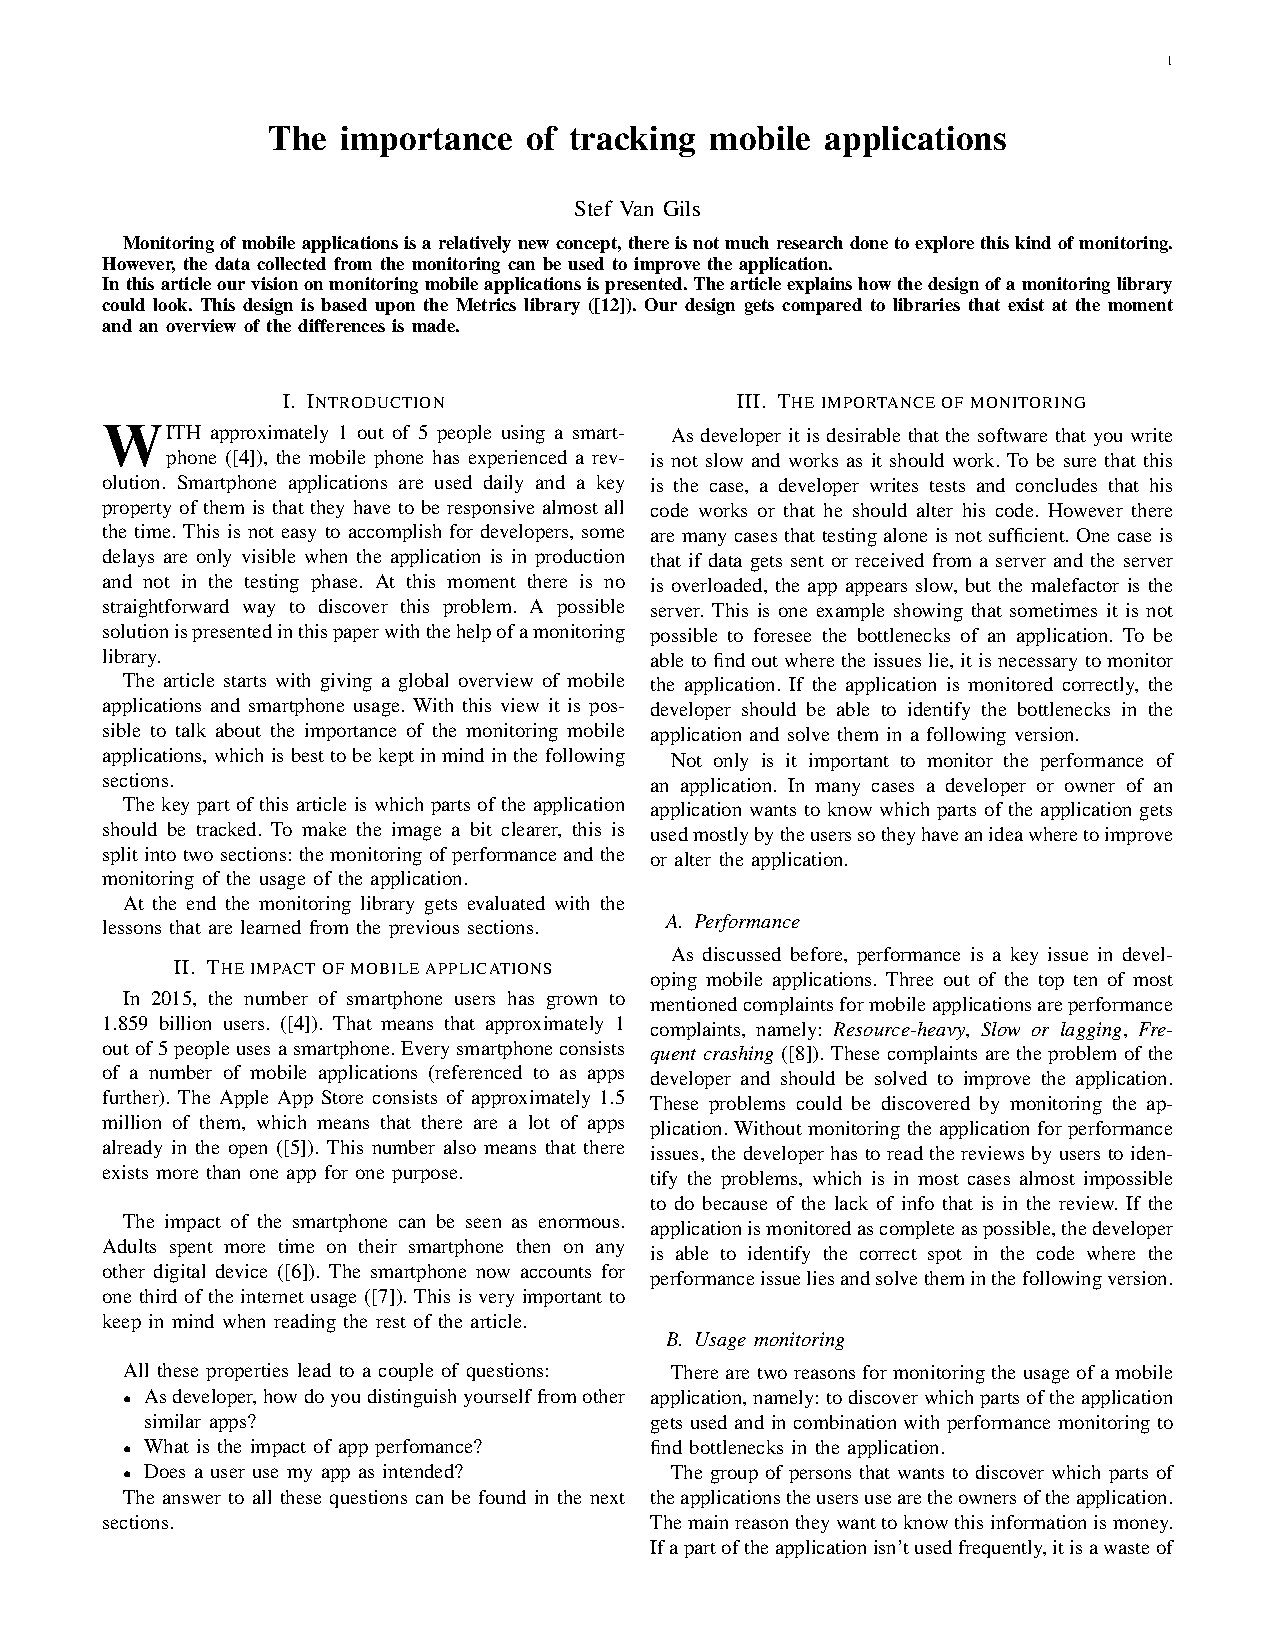
\includepdf[pages={1-5}]{article_thesis}
% ... en zo verder tot
%\chapter{De laatste bijlage}
\label{app:n}
In de bijlagen vindt men de data terug die nuttig kunnen zijn voor de
lezer, maar die niet essentieel zijn om het betoog in de normale tekst te
kunnen volgen. Voorbeelden hiervan zijn bronbestanden,
configuratie-informatie, langdradige wiskundige afleidingen, enz.

\section{Lorem 20-24}
\lipsum[20-24]

\section{Lorem 25-27}
\lipsum[25-27]

%%% Local Variables: 
%%% mode: latex
%%% TeX-master: "masterproef"
%%% End: 


\backmatter
% Na de bijlagen plaatst men nog de bibliografie.
% Je kan de  standaard "abbrv" bibliografiestijl vervangen door een andere.
\bibliographystyle{abbrv}
\bibliography{referenties}



\end{document}

%%% Local Variables: 
%%% mode: latex
%%% TeX-master: t
%%% End: 
